\section{Specifications}
\label{sec:Specifications}

\newcounter{rulei}[subsection]
\newcommand{\rcnii}{\stepcounter{rulei}\arabic{section}.\arabic{subsection}.\arabic{rulei}}
\renewcommand{\labelenumi}{\rcnii}

\subsection{Markers}
\label{sub:markers}
The arena, tokens, buckets, and robots involved in the game are labelled with \textit{libkoki} markers.  Each marker pattern encodes a number.  Each marker number is associated with a particular feature within the arena, and also has an associated size.  The marker numbers and sizes are as follows:

\begin{center}
  \begin{tabular}{lcc}
    \toprule
    \textbf{Item} & \textbf{Marker Numbers} & \textbf{Marker Size (mm)} \\
    \midrule
    Arena boundary & 0 -- 27 & 250 \\
    Robots & 28 -- 31 & 100 \\
    Tokens & 32 -- 71 & 100 \\
    Bucket side & 72 -- 75 & 100 \\
    Bucket end & 76 -- 79 & 100 \\
    \bottomrule
  \end{tabular}
\end{center}

Two sets of marker codes will be used: one for development purpose, and one for the competition itself.  The competition set is only to be used inside the Student Robotics arena at the Student Robotics competition.  This is so that people carrying markers past the arena do not confuse robots.  The competition codes are 100 above the development codes.  When run in competition mode (specifiable through the robot's GUI), the software provided by Student Robotics will subtract 100 from the detected marker codes, as well as ignore the development codes.

The markers can be printed on a black-and-white printer.  Marker designs can be downloaded from the documentation section of the Student Robotics website.

Unless specified otherwise, all markers described in this document are oriented vertically such that the principle corner of the marker (which is indicated by a dark grey dot in the black marker border) is on the higher edge.

\subsection{Arena}
\label{sub:arena}
\begin{enumerate}
\item The match arena floor, overall, is an $8m \times 8m$ square, as shown in figure~\ref{fig:arena-dim}.  The tolerance of these two dimensions is $\pm0.25m$.

\begin{figure}
  \centering
  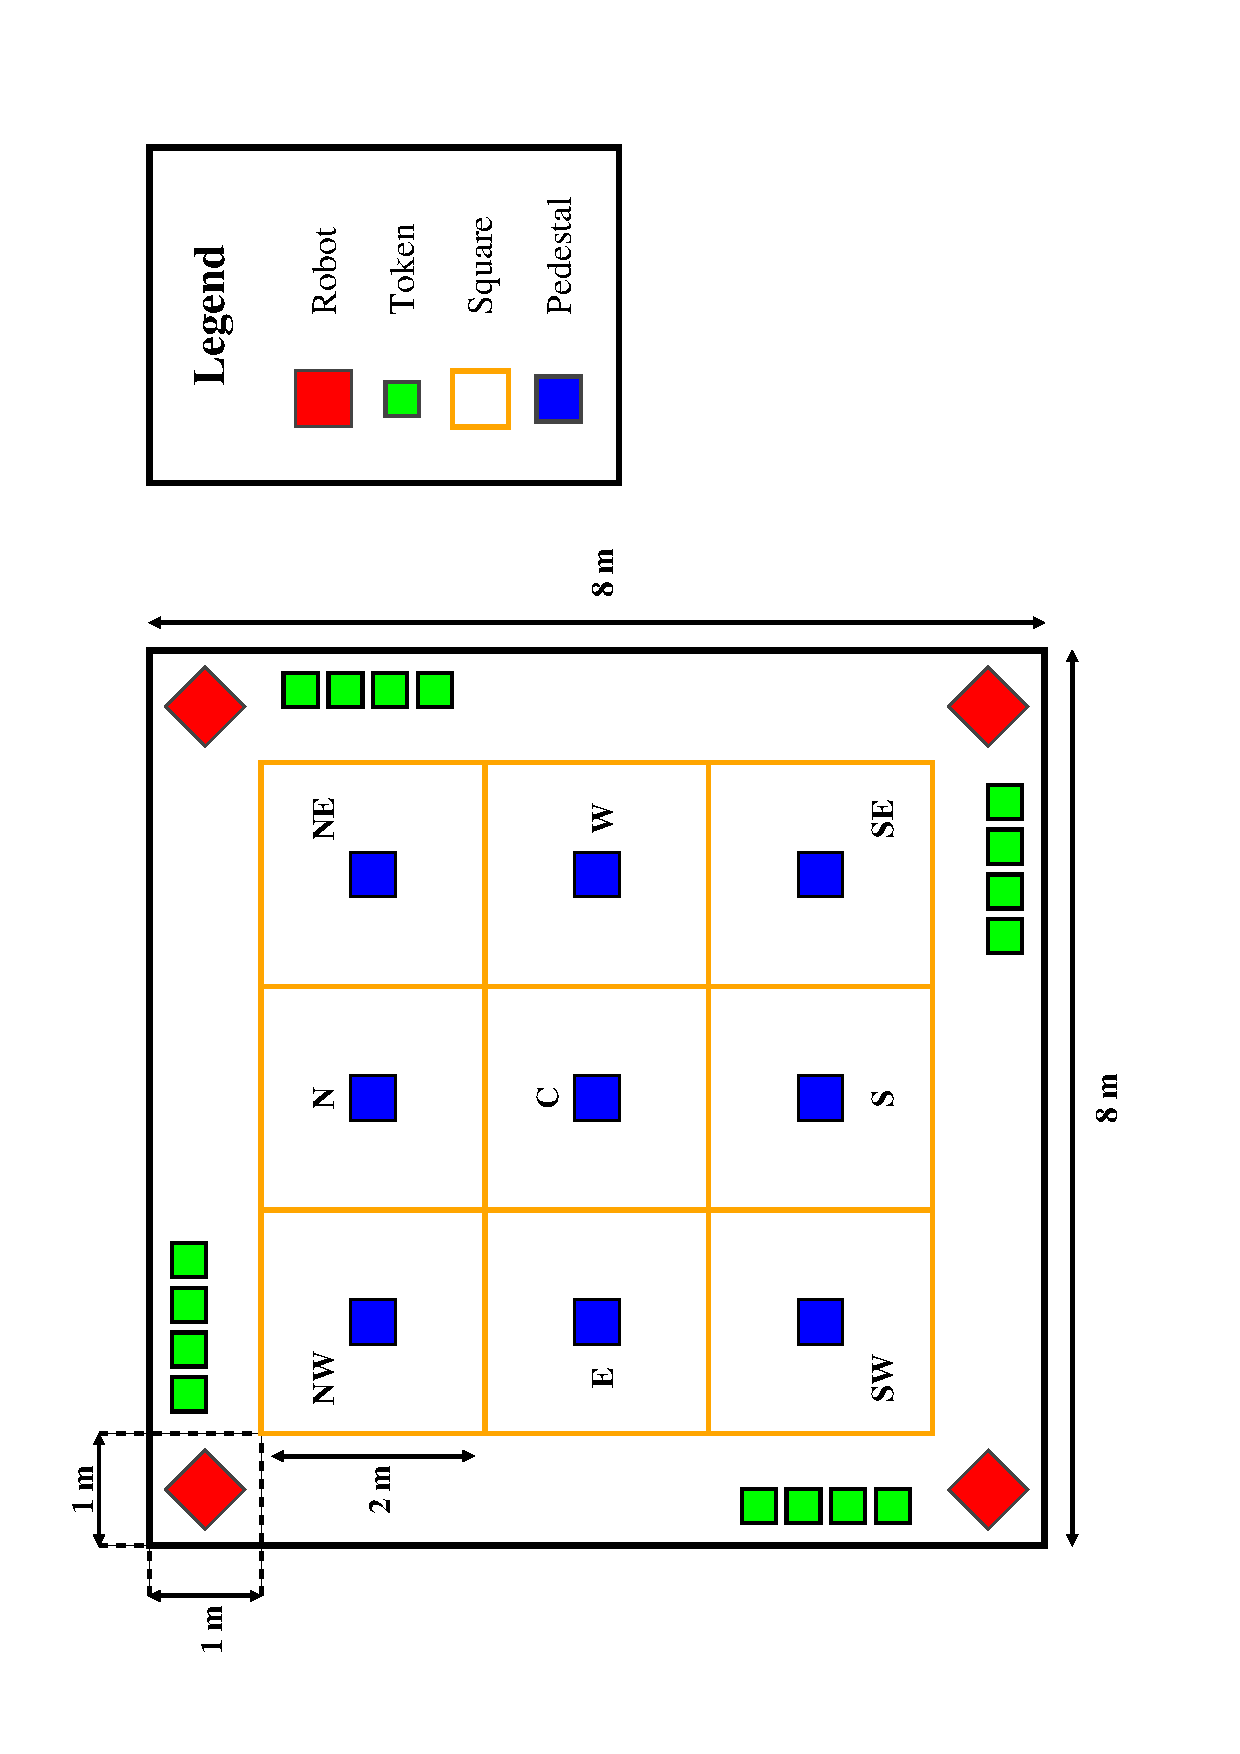
\includegraphics[width=0.8\textwidth]{./images/arena.pdf}
  \caption{\label{fig:arena-dim}A bird's-eye view of the arena.}
\end{figure}

\item The ``bucket barrier'' is a horizontal bar arranged in a $6m \times 6m$ square centred and aligned with the boundary of the arena.  The lower edge of the barrier is $750mm$ above the floor.

\item The bucket barrier is suspended by eight legs, each of which has a maximum footprint of $150mm \times 200mm$.  These footprints extend into the centre of the arena, and are flush with the outer side of the bucker barrier.

  \begin{figure}
    \centering
    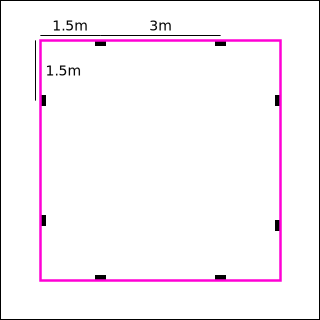
\includegraphics{./images/barrier-feet.pdf}
    \caption{The positions of the posts supporting the bucket barrier.}
    \label{fig:bucker-barrier-legs}
  \end{figure}

\item The floor of the arena is carpeted.  The carpet tiles used in the arena are from B\&Q, with EAN 5014957151543.

\item The arena walls are $600\pm30mm$ high, the interior surfaces of which are white plastic-coated hardboard.

\item The arena features four \textit{zones}.  These areas are delineated by the boundary of the arena, the bucket barrier, and lines between the corners of the arena and bucket barrier.  The numbering of these zones is shown in figure~\ref{fig:arena-zones}.

  \begin{figure}
    \centering
    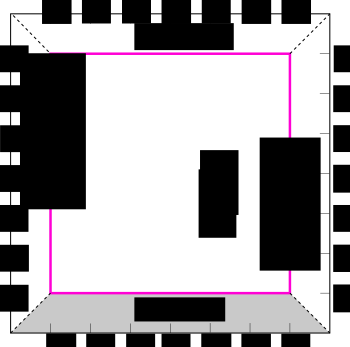
\includegraphics{./images/arena-markers.pdf}
    \caption{The positions of the four zones in the arena.  The shaded area forms zone 1, and the other zones are rotationally symmetric to this.  The numbers shown around the perimeter of this diagram are the numbers of the markers positioned on the wall.}
    \label{fig:arena-zones}
  \end{figure}

\item Each wall of the arena features seven $250mm$ libkoki markers.  Figure~\ref{fig:arena-wall} shows the positioning of these markers, whilst figure~\ref{fig:arena-zones} shows the numbering of these markers.

  \begin{figure}
    \centering
    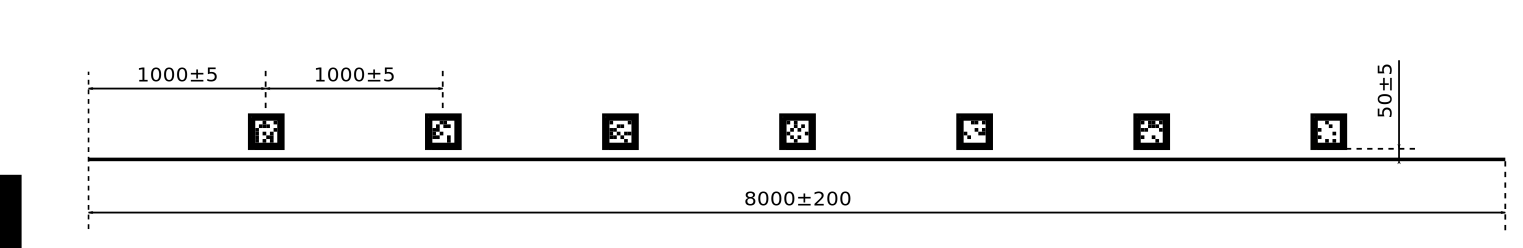
\includegraphics[width=\textwidth]{./images/sidewall.pdf}
    \caption{Seven $250mm$ wide markers are spaced evenly along each $8m$ arena wall.  The markers are placed $50mm$ above the floor.}
    \label{fig:arena-wall}
  \end{figure}

\end{enumerate}

\subsection{Tokens}
\label{sub:Tokens}
\begin {enumerate}
\item Tokens are cubic corrugated cardboard boxes with side $102 \pm TODO mm$.
\emph{Each team's kit contains four of these.}
\item Tokens have a mass of $475\pm30g$.
\end {enumerate}

\subsection{Buckets}
\label{sub:buckets}
\begin{figure}
  \centering
  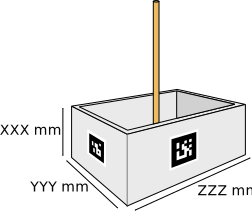
\includegraphics{./images/bucket-3d.pdf}
  \caption{Dimensions of the bucket.}
  \label{fig:bucket-3d}
\end{figure}

\begin{enumerate}
\item Buckets are cuboid structures with the dimensions shown in figure~\ref{fig:bucket-3d}.  Casters are mounted on the underside of the buckets, allowing the bucket to be pushed or pulled around.  \textit{A guide on how to assemble a bucket, and where to get suitable parts can be found on the Student Robotics website.}

\item A TODO long, $15mm$ diameter wooden dowel pole extends vertically from the centre of the bucket.  Combined with the bucket barrier, this prevents buckets from entering the central area of the arena.

\item Each bucket features two marker numbers: one which is used on the shorter sides of the bucket (a.k.a. ``the bucket ends''), and one that is used on the other vertical sides of the bucket.  These markers are $100mm$ in width, and are placed in the centre of the bucket faces that they occupy.

\end{enumerate}

\clearpage
